\section{UML MODELS}
\subsection{Use case diagram}
\begin{figure}[H]
	\centering
	\includegraphics[width=14cm]{UseCase}
\end{figure}
\newpage
\subsection{Use case description}
In this paragraph all our use cases are described.
\begin{itemize}
	\item User registration by filling out a form [\hyperlink{UserRegistration}{Sequence Diagram}]:
	\begin{table}[H]
		\centering
		\begin{tabular}{| m{3.5cm} | m{9.5cm} |}
			\hline
			\textbf{Name} & User: registration, fill out a registration form, first login\\
			\hline
			\textbf{Actors} & Generic user\\
			\hline
			\textbf{Entry conditions} & There are no entry conditions.\\
			\hline
			\textbf{Flow of Events} & 
			\begin{enumerate}
				\item The user downloads the mobile application or accesses the service's website.
				\item The user clicks on the "Sign in" button.
				\item The user enters his credentials and payment information.
				\item The user clicks again on the "Sign in" button.
				\item The user receives a password via email.
			\end{enumerate} \\
			\hline
			\textbf{Exit conditions} & The user makes his first login with the assigned password and the username he chose.\\
			\hline
			\textbf{Exceptions} & The username is already taken or the user did not fill in all the mandatory fields. \\
			\hline
		\end{tabular}
	\end{table}
		\item Registered user login [\hyperlink{Login}{Sequence Diagram}]:
	\begin{table}[H]
		\centering
		\begin{tabular}{| m{3.5cm} | m{9.5cm} |}
			\hline
			\textbf{Name} & Registered user: login\\
			\hline
			\textbf{Actors} & Registered user\\
			\hline
			\textbf{Entry conditions} & The registered user has previously registered to the system.\\
			\hline
			\textbf{Flow of Events} & 
			\begin{enumerate}
				\item The registered user accesses the service's website or opens the mobile application.
				\item The registered user enters his credentials into the corresponding fields.
				\item The registered user clicks on the "Login" button.
			\end{enumerate} \\
			\hline
			\textbf{Exit conditions} & The registered user is able to see his personal page.\\
			\hline
			\textbf{Exceptions} & The username-password combination does not exist into the database. \\
			\hline
		\end{tabular}
	\end{table}
\newpage
	\item Registered user views his profile [\hyperlink{ViewProfile}{Sequence Diagram}]:
	\begin{table}[H]
		\centering
		\begin{tabular}{| m{3.5cm} | m{9.5cm} |}
			\hline
			\textbf{Name} & Registered user: view profile\\
			\hline
			\textbf{Actors} & Registered user\\
			\hline
			\textbf{Entry conditions} & The registered user has previously logged into the system.\\
			\hline
			\textbf{Flow of Events} & 
			\begin{enumerate}
				\item The registered user accesses his profile by clicking on the "View your profile" button.
			\end{enumerate} \\
			\hline
			\textbf{Exit conditions} & The registered user is able to see his profile page.\\
			\hline
			\textbf{Exceptions} & Wrong button clicked. \\
			\hline
		\end{tabular}
	\end{table}
\item Registered user manages his personal information [\hyperlink{ManageInfo}{Sequence Diagram}]:
\begin{table}[H]
	\centering
	\begin{tabular}{| m{3.5cm} | m{9.5cm} |}
		\hline
		\textbf{Name} & Registered user: manage personal information\\
		\hline
		\textbf{Actors} & Registered user\\
		\hline
		\textbf{Entry conditions} & The registered user has previously logged into the system.\\
		\hline
		\textbf{Flow of Events} & 
		\begin{enumerate}
			\item The registered user accesses his profile by clicking on the "View your profile" button.
			\item The registered user can modify his personal information by clicking on the "Manage personal information" button.
			\item The registered user makes some changes (or none).
			\item The registered user clicks on the "Save changes" button.  
		\end{enumerate} \\
		\hline
		\textbf{Exit conditions} & The registered user's personal information is updated.\\
		\hline
		\textbf{Exceptions} & Wrong data entered. \\
		\hline
	\end{tabular}
\end{table}
\newpage
\item Registered user cancels his current reservation [\hyperlink{CancelRes}{Sequence Diagram}]:
\begin{table}[H]
	\centering
	\begin{tabular}{| m{3.5cm} | m{9.5cm} |}
		\hline
		\textbf{Name} & Registered user: cancel reservation\\
		\hline
		\textbf{Actors} & Registered user\\
		\hline
		\textbf{Entry conditions} & The registered user has previously logged into the system.\\
		\hline
		\textbf{Flow of Events} & 
		\begin{enumerate}
			\item The registered user clicks on the "View the list of your reservations" button.
			\item The registered user visualizes the page showing all his reservations.
			\item The registered user clicks on the "Cancel current reservation" button.
		\end{enumerate} \\
		\hline
		\textbf{Exit conditions} & The registered user's current reservation no longer exists and is added to the past reservations' list labeled as "Deleted".\\
		\hline
		\textbf{Exceptions} & The registered user has no current or past reservations.\\
		\hline
	\end{tabular}
\end{table}
\newpage
\item Registered user reports an issue after unlocking the car [\hyperlink{ReportIssue}{Sequence Diagram}]:
\begin{table}[H]
	\centering
	\begin{tabular}{| m{3.5cm} | m{9.5cm} |}
		\hline
		\textbf{Name} & Registered user: unlock car, report issue\\
		\hline
		\textbf{Actors} & Registered user\\
		\hline
		\textbf{Entry conditions} & The registered user has previously logged into the system, made a reservation and selected a car.\\
		\hline
		\textbf{Flow of Events} & 
		\begin{enumerate}
			\item The registered user visualizes the list of his previous and current reservations from his personal page.
			\item The registered user clicks on the "Unlock car" button next to his current reservation.
			\item The registered user visualizes the car's information.
			\item The registered user checks the car for possible issues.
			\item The registered user clicks on the "Report issue" button.   
		\end{enumerate} \\
		\hline
		\textbf{Exit conditions} & The registered user's current reservation is deleted and he/she receives an email saying that an employee will be sent to take care of the car.\\
		\hline
		\textbf{Exceptions} & The car presents no issues.\\
		\hline
	\end{tabular}
\end{table}
\newpage
\item Registered user makes a reservation by selecting a car [\hyperlink{Reservation}{Sequence Diagram}]:
\begin{table}[H]
	\centering
	\begin{tabular}{| m{3.5cm} | m{9.5cm} |}
		\hline
		\textbf{Name} & Registered user: make reservation, insert specific address/current location, select available car\\
		\hline
		\textbf{Actors} & Registered user\\
		\hline
		\textbf{Entry conditions} & The registered user has previously logged into the system.\\
		\hline
		\textbf{Flow of Events} & 
		\begin{enumerate}
			\item The registered user clicks on the "Click here" button from his personal page.
			\item The registered user enters a valid address or lets the system track his position by clicking on the "Track my position" button.
			\item The registered user visualizes all the available cars on a map.
			\item The registered user chooses one of the available cars shown on the map.
			\item The registered user clicks on the "Continue" button to reserve the car.   
		\end{enumerate} \\
		\hline
		\textbf{Exit conditions} & The registered user is able to see the page with all his previous and current reservations.\\
		\hline
		\textbf{Exceptions} & A non valid address is entered. None of the available cars is selected by the registered user. The registered user's GPS is not active although he has chosen the "Track my position" option.\\
		\hline
	\end{tabular}
\end{table}
\newpage
\item Employee logs into the system and manages a car's information [\hyperlink{EmployeeManageCarInfo}{Sequence Diagram}]:
\begin{table}[H]
	\centering
	\begin{tabular}{| m{3.5cm} | m{9.5cm} |}
		\hline
		\textbf{Name} & Employee: login, manage car information\\
		\hline
		\textbf{Actors} & Employee\\
		\hline
		\textbf{Entry conditions} & The employee has previously been added to the database.\\
		\hline
		\textbf{Flow of Events} & 
		\begin{enumerate}
			\item The employee opens the website homepage.
			\item The employee logs into the system by providing his/her credentials.
			\item The employee visualizes the list of all PowerEnJoy cars.
			\item The employee selects a car directly from the list or by searching its plate.
			\item The employee visualizes the chosen car's information.
			\item The employee manages the car's information. 
			\item The employee clicks on the "Save changes" button.  
		\end{enumerate} \\
		\hline
		\textbf{Exit conditions} & The car's information is changed and the employee visualizes the list of all PowerEnJoy cars.\\
		\hline
		\textbf{Exceptions} & Wrong credentials are given. The searched plate does not exist. Non valid values are entered into the car's information fields.\\
		\hline
	\end{tabular}
\end{table}
\end{itemize}
\subsection{Class diagram}
\begin{figure}[H]
	\centering
	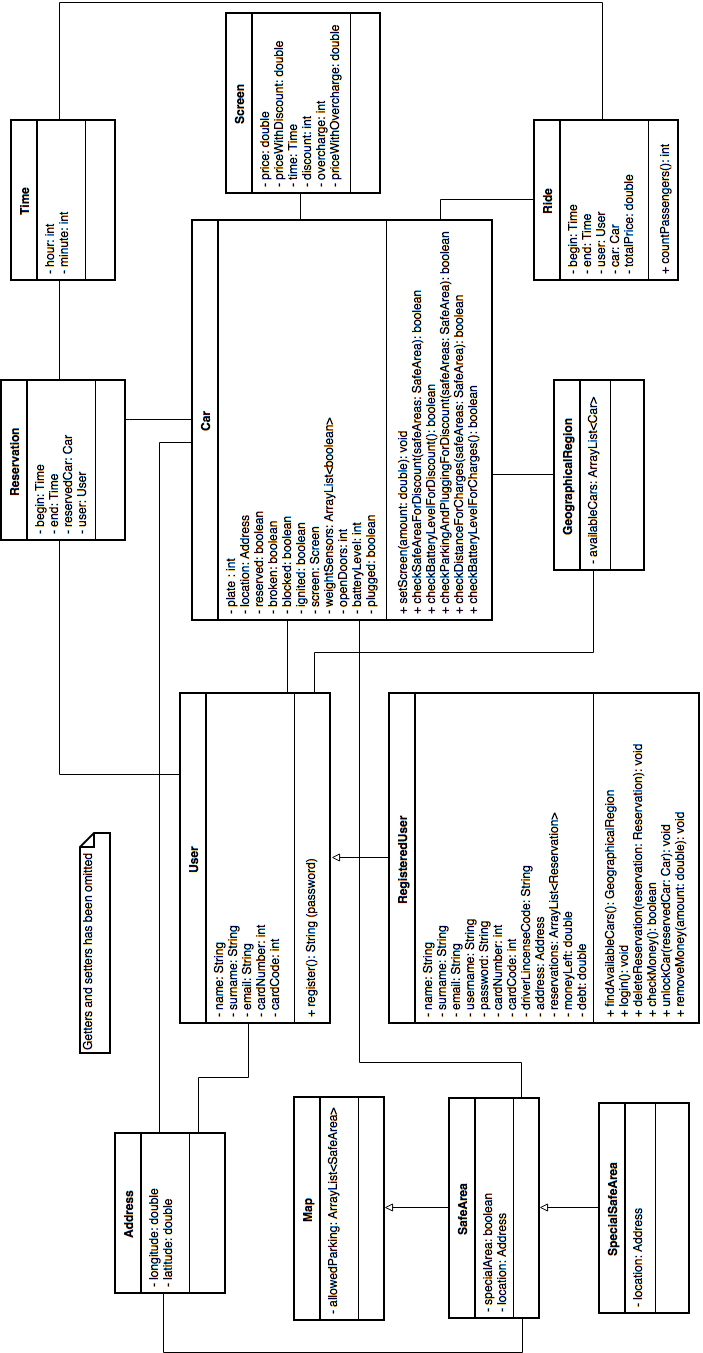
\includegraphics[height=19.5cm]{Class_diagram}
\end{figure}
\subsection{Sequence diagrams}
\begin{itemize}
	\item \hypertarget{UserRegistration} User's registration:
	\begin{figure}[H]
		\centering
		\includegraphics[height=19cm]{UserRegistration}
	\end{figure}
\item \hypertarget{Login} Registered user login:
\begin{figure}[H]
	\centering
	\includegraphics[width=14cm]{Login}
\end{figure}
\newpage
\item \hypertarget{ViewProfile} Registered user views his profile:
\begin{figure}[H]
	\centering
	\includegraphics[width=14cm]{ViewProfile}
\end{figure}
\item \hypertarget{ManageInfo} Registered user manages his personal information:
\begin{figure}[H]
	\centering
	\includegraphics[width=14cm]{ManageInfo}
\end{figure}
\item \hypertarget{Reservation} Registered user makes a reservation by selecting a car:
\begin{figure}[H]
	\centering
	\includegraphics[height=19.5cm]{Reservation}
\end{figure}
\item \hypertarget{ReportIssue} Registered user reports an issue after unlocking the car:
\begin{figure}[H]
	\centering
	\includegraphics[width=13.5cm]{ReportIssue}
\end{figure}
\newpage
\item \hypertarget{CancelRes} Registered user cancels his current reservation:
\begin{figure}[H]
	\centering
	\includegraphics[width=14cm]{CancelRes}
\end{figure}
\newpage
\item \hypertarget{EmployeeManageCarInfo} Employee manages car's information:
\begin{figure}[H]
	\centering
	\includegraphics[height=19.5cm]{EmployeeManageCarInfo}
\end{figure}
\end{itemize}
\newpage
\subsection{Activity diagram}
User's registration by filling out a form:
\begin{figure}[H]
	\centering
	\includegraphics[width=14.5cm]{ActivityDiagram}
\end{figure}
\subsection{State diagram}
Reservation:
\begin{figure}[H]
	\centering
	\includegraphics[width=14.5cm]{StateDiagram}
\end{figure}